\documentclass{standalone}
\usepackage{tikz}
\usetikzlibrary{patterns, positioning}

\begin{document}
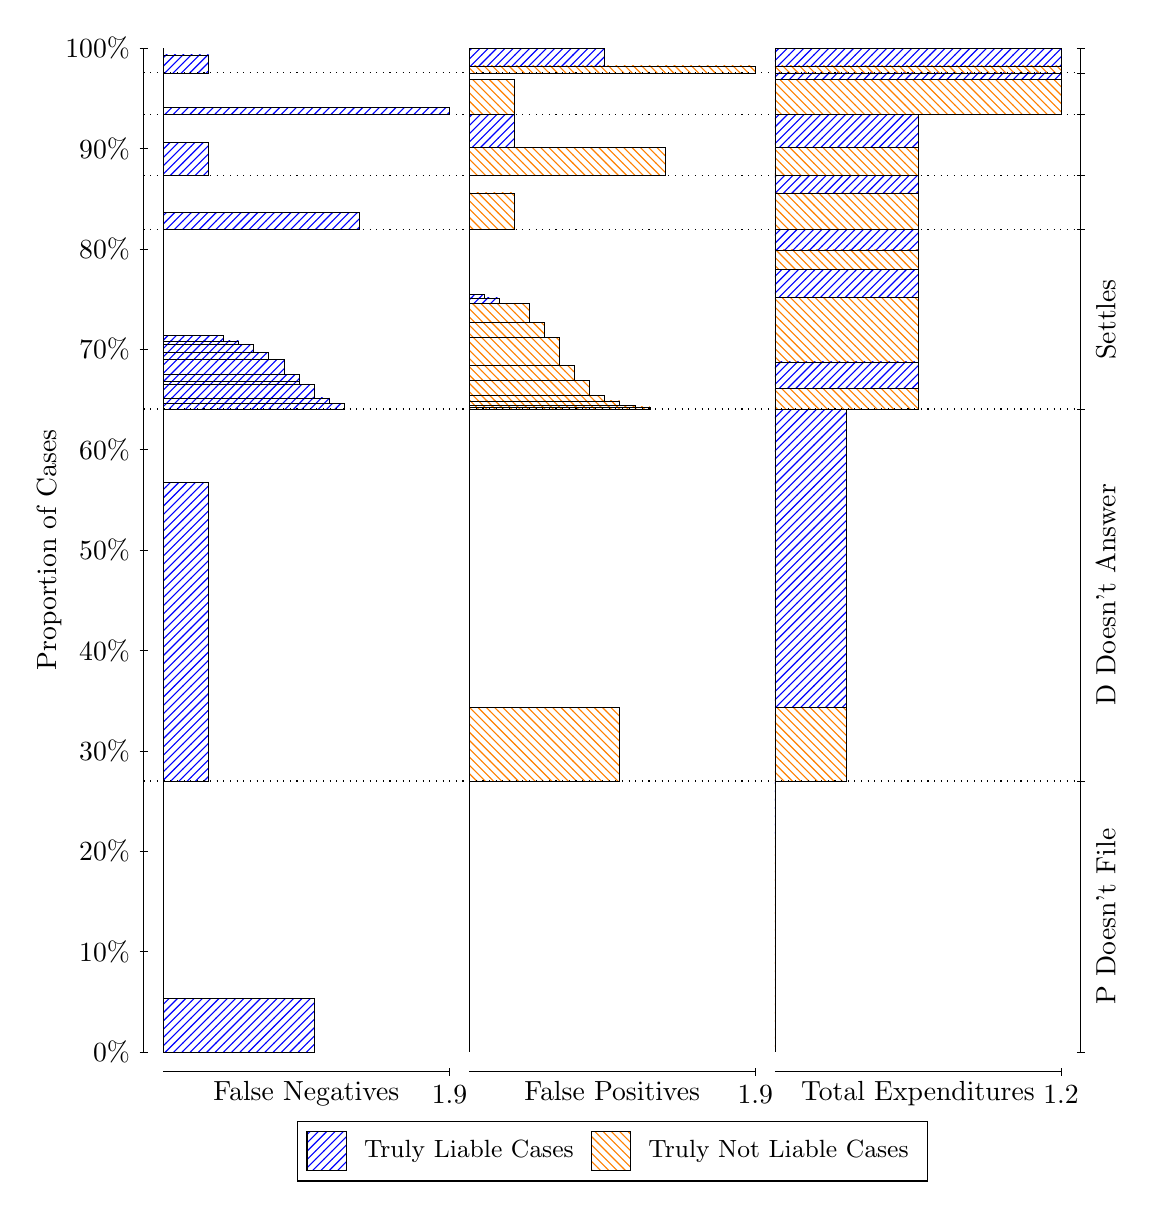
\begin{tikzpicture}
\draw[black, very thin] (1.5,1.75) -- (1.5,14.5);
\node[rotate=90, anchor=center] at (0.3, 8.125) {Proportion of Cases};
\draw[black, very thin] (1.45,1.75) -- (1.55,1.75);
\node[anchor=east] at (1.45, 1.75) {0\%};
\draw[black, very thin] (1.45,3.025) -- (1.55,3.025);
\node[anchor=east] at (1.45, 3.025) {10\%};
\draw[black, very thin] (1.45,4.3) -- (1.55,4.3);
\node[anchor=east] at (1.45, 4.3) {20\%};
\draw[black, very thin] (1.45,5.575) -- (1.55,5.575);
\node[anchor=east] at (1.45, 5.575) {30\%};
\draw[black, very thin] (1.45,6.85) -- (1.55,6.85);
\node[anchor=east] at (1.45, 6.85) {40\%};
\draw[black, very thin] (1.45,8.125) -- (1.55,8.125);
\node[anchor=east] at (1.45, 8.125) {50\%};
\draw[black, very thin] (1.45,9.4) -- (1.55,9.4);
\node[anchor=east] at (1.45, 9.4) {60\%};
\draw[black, very thin] (1.45,10.675) -- (1.55,10.675);
\node[anchor=east] at (1.45, 10.675) {70\%};
\draw[black, very thin] (1.45,11.95) -- (1.55,11.95);
\node[anchor=east] at (1.45, 11.95) {80\%};
\draw[black, very thin] (1.45,13.225) -- (1.55,13.225);
\node[anchor=east] at (1.45, 13.225) {90\%};
\draw[black, very thin] (1.45,14.5) -- (1.55,14.5);
\node[anchor=east] at (1.45, 14.5) {100\%};

\draw[black, very thin] (13.4,1.75) -- (13.4,14.5);
\draw[black, very thin] (13.35,1.75) -- (13.45,1.75);
\node[anchor=west] at (13.35, 1.75) {};
\draw[black, very thin] (13.35,5.1907) -- (13.45,5.1907);
\node[anchor=west] at (13.35, 5.1907) {};
\draw[black, very thin] (13.35,9.9155) -- (13.45,9.9155);
\node[anchor=west] at (13.35, 9.9155) {};
\draw[black, very thin] (13.35,12.193) -- (13.45,12.193);
\node[anchor=west] at (13.35, 12.193) {};
\draw[black, very thin] (13.35,12.878) -- (13.45,12.878);
\node[anchor=west] at (13.35, 12.878) {};
\draw[black, very thin] (13.35,13.661) -- (13.45,13.661);
\node[anchor=west] at (13.35, 13.661) {};
\draw[black, very thin] (13.35,14.185) -- (13.45,14.185);
\node[anchor=west] at (13.35, 14.185) {};
\draw[black, very thin] (13.35,14.5) -- (13.45,14.5);
\node[anchor=west] at (13.35, 14.5) {};

\draw[black, very thin, pattern color=blue, pattern=north east lines] (1.75,1.75) rectangle (3.6623,2.4337);
\draw[black, very thin, pattern color=orange, pattern=north west lines] (1.75,2.4337) rectangle (1.75,5.1907);
\draw[black, very thin, pattern color=blue, pattern=north east lines] (1.75,5.1907) rectangle (2.3237,8.9836);
\draw[black, very thin, pattern color=orange, pattern=north west lines] (1.75,8.9836) rectangle (1.75,9.9155);
\draw[black, very thin, pattern color=blue, pattern=north east lines] (1.75,9.9155) rectangle (4.0447,9.9833);
\draw[black, very thin, pattern color=blue, pattern=north east lines] (1.75,9.9833) rectangle (3.8535,10.058);
\draw[black, very thin, pattern color=blue, pattern=north east lines] (1.75,10.058) rectangle (3.6623,10.229);
\draw[black, very thin, pattern color=blue, pattern=north east lines] (1.75,10.229) rectangle (3.4711,10.263);
\draw[black, very thin, pattern color=blue, pattern=north east lines] (1.75,10.263) rectangle (3.4711,10.36);
\draw[black, very thin, pattern color=blue, pattern=north east lines] (1.75,10.36) rectangle (3.2798,10.545);
\draw[black, very thin, pattern color=blue, pattern=north east lines] (1.75,10.545) rectangle (3.0886,10.634);
\draw[black, very thin, pattern color=blue, pattern=north east lines] (1.75,10.634) rectangle (2.8974,10.735);
\draw[black, very thin, pattern color=blue, pattern=north east lines] (1.75,10.735) rectangle (2.7061,10.781);
\draw[black, very thin, pattern color=blue, pattern=north east lines] (1.75,10.781) rectangle (2.5149,10.852);
\draw[black, very thin, pattern color=orange, pattern=north west lines] (1.75,10.852) rectangle (1.75,12.193);
\draw[black, very thin, pattern color=blue, pattern=north east lines] (1.75,12.193) rectangle (4.236,12.412);
\draw[black, very thin, pattern color=orange, pattern=north west lines] (1.75,12.412) rectangle (1.75,12.878);
\draw[black, very thin, pattern color=blue, pattern=north east lines] (1.75,12.878) rectangle (2.3237,13.305);
\draw[black, very thin, pattern color=orange, pattern=north west lines] (1.75,13.305) rectangle (1.75,13.661);
\draw[black, very thin, pattern color=blue, pattern=north east lines] (1.75,13.661) rectangle (5.3833,13.749);
\draw[black, very thin, pattern color=orange, pattern=north west lines] (1.75,13.749) rectangle (1.75,14.185);
\draw[black, very thin, pattern color=blue, pattern=north east lines] (1.75,14.185) rectangle (2.3237,14.413);
\draw[black, very thin, pattern color=orange, pattern=north west lines] (1.75,14.413) rectangle (1.75,14.5);
\draw[black, very thin, pattern color=orange, pattern=north west lines] (5.6333,1.75) rectangle (5.6333,4.507);
\draw[black, very thin, pattern color=blue, pattern=north east lines] (5.6333,4.507) rectangle (5.6333,5.1907);
\draw[black, very thin, pattern color=orange, pattern=north west lines] (5.6333,5.1907) rectangle (7.5456,6.1226);
\draw[black, very thin, pattern color=blue, pattern=north east lines] (5.6333,6.1226) rectangle (5.6333,9.9155);
\draw[black, very thin, pattern color=orange, pattern=north west lines] (5.6333,9.9155) rectangle (7.9281,9.9412);
\draw[black, very thin, pattern color=orange, pattern=north west lines] (5.6333,9.9412) rectangle (7.7368,9.9637);
\draw[black, very thin, pattern color=orange, pattern=north west lines] (5.6333,9.9637) rectangle (7.5456,10.018);
\draw[black, very thin, pattern color=orange, pattern=north west lines] (5.6333,10.018) rectangle (7.3544,10.091);
\draw[black, very thin, pattern color=orange, pattern=north west lines] (5.6333,10.091) rectangle (7.1632,10.281);
\draw[black, very thin, pattern color=orange, pattern=north west lines] (5.6333,10.281) rectangle (6.9719,10.471);
\draw[black, very thin, pattern color=orange, pattern=north west lines] (5.6333,10.471) rectangle (6.7807,10.828);
\draw[black, very thin, pattern color=orange, pattern=north west lines] (5.6333,10.828) rectangle (6.5895,11.016);
\draw[black, very thin, pattern color=orange, pattern=north west lines] (5.6333,11.016) rectangle (6.3982,11.256);
\draw[black, very thin, pattern color=blue, pattern=north east lines] (5.6333,11.256) rectangle (6.0158,11.327);
\draw[black, very thin, pattern color=blue, pattern=north east lines] (5.6333,11.327) rectangle (5.8246,11.374);
\draw[black, very thin, pattern color=blue, pattern=north east lines] (5.6333,11.374) rectangle (5.6333,12.193);
\draw[black, very thin, pattern color=orange, pattern=north west lines] (5.6333,12.193) rectangle (6.207,12.659);
\draw[black, very thin, pattern color=blue, pattern=north east lines] (5.6333,12.659) rectangle (5.6333,12.878);
\draw[black, very thin, pattern color=orange, pattern=north west lines] (5.6333,12.878) rectangle (8.1193,13.234);
\draw[black, very thin, pattern color=blue, pattern=north east lines] (5.6333,13.234) rectangle (6.207,13.661);
\draw[black, very thin, pattern color=orange, pattern=north west lines] (5.6333,13.661) rectangle (6.207,14.097);
\draw[black, very thin, pattern color=blue, pattern=north east lines] (5.6333,14.097) rectangle (5.6333,14.185);
\draw[black, very thin, pattern color=orange, pattern=north west lines] (5.6333,14.185) rectangle (9.2667,14.272);
\draw[black, very thin, pattern color=blue, pattern=north east lines] (5.6333,14.272) rectangle (7.3544,14.5);
\draw[black, very thin, pattern color=orange, pattern=north west lines] (9.5167,1.75) rectangle (9.5167,4.507);
\draw[black, very thin, pattern color=blue, pattern=north east lines] (9.5167,4.507) rectangle (9.5167,5.1907);
\draw[black, very thin, pattern color=orange, pattern=north west lines] (9.5167,5.1907) rectangle (10.425,6.1226);
\draw[black, very thin, pattern color=blue, pattern=north east lines] (9.5167,6.1226) rectangle (10.425,9.9155);
\draw[black, very thin, pattern color=orange, pattern=north west lines] (9.5167,9.9155) rectangle (11.333,10.182);
\draw[black, very thin, pattern color=blue, pattern=north east lines] (9.5167,10.182) rectangle (11.333,10.514);
\draw[black, very thin, pattern color=orange, pattern=north west lines] (9.5167,10.514) rectangle (11.333,11.338);
\draw[black, very thin, pattern color=blue, pattern=north east lines] (9.5167,11.338) rectangle (11.333,11.685);
\draw[black, very thin, pattern color=orange, pattern=north west lines] (9.5167,11.685) rectangle (11.333,11.936);
\draw[black, very thin, pattern color=blue, pattern=north east lines] (9.5167,11.936) rectangle (11.333,12.193);
\draw[black, very thin, pattern color=orange, pattern=north west lines] (9.5167,12.193) rectangle (11.333,12.659);
\draw[black, very thin, pattern color=blue, pattern=north east lines] (9.5167,12.659) rectangle (11.333,12.878);
\draw[black, very thin, pattern color=orange, pattern=north west lines] (9.5167,12.878) rectangle (11.333,13.234);
\draw[black, very thin, pattern color=blue, pattern=north east lines] (9.5167,13.234) rectangle (11.333,13.661);
\draw[black, very thin, pattern color=orange, pattern=north west lines] (9.5167,13.661) rectangle (13.15,14.097);
\draw[black, very thin, pattern color=blue, pattern=north east lines] (9.5167,14.097) rectangle (13.15,14.185);
\draw[black, very thin, pattern color=orange, pattern=north west lines] (9.5167,14.185) rectangle (13.15,14.272);
\draw[black, very thin, pattern color=blue, pattern=north east lines] (9.5167,14.272) rectangle (13.15,14.5);
\draw[black, dotted] (1.5,5.1907) -- (13.4,5.1907);
\draw[black, dotted] (1.5,9.9155) -- (13.4,9.9155);
\draw[black, dotted] (1.5,12.193) -- (13.4,12.193);
\draw[black, dotted] (1.5,12.878) -- (13.4,12.878);
\draw[black, dotted] (1.5,13.661) -- (13.4,13.661);
\draw[black, dotted] (1.5,14.185) -- (13.4,14.185);
\draw[black, very thin] (1.75,1.5) -- (5.3833,1.5);
\node[anchor=north] at (3.5667, 1.5) {False Negatives};
\draw[black, very thin] (5.3833,1.45) -- (5.3833,1.55);
\node[anchor=north] at (5.3833, 1.45) {1.9};

\draw[black, very thin] (5.6333,1.5) -- (9.2667,1.5);
\node[anchor=north] at (7.45, 1.5) {False Positives};
\draw[black, very thin] (9.2667,1.45) -- (9.2667,1.55);
\node[anchor=north] at (9.2667, 1.45) {1.9};

\draw[black, very thin] (9.5167,1.5) -- (13.15,1.5);
\node[anchor=north] at (11.333, 1.5) {Total Expenditures};
\draw[black, very thin] (13.15,1.45) -- (13.15,1.55);
\node[anchor=north] at (13.15, 1.45) {1.2};

\node[black, centered, rotate=90] at (13.72, 3.4703) {P Doesn't File};
\node[black, centered, rotate=90] at (13.72, 7.5531) {D Doesn't Answer};
\node[black, centered, rotate=90] at (13.72, 11.054) {Settles};





\draw (7.449999999999999,1.5) node[draw=none] (baseCoordinate) {};
\begin{scope}[align=center]
        \matrix[scale=0.5, draw=black, below=0.5cm of baseCoordinate, nodes={draw}, column sep=0.1cm]{
            \node[rectangle, draw, minimum width=0.5cm, minimum height=0.5cm, pattern=north east lines, pattern color=blue] {}; &
            \node[draw=none, font=\small] (B) {Truly Liable Cases}; &
            \node[rectangle, draw, minimum width=0.5cm, minimum height=0.5cm, pattern=north west lines, pattern color=orange] {}; &
            \node[draw=none, font=\small] (B) {Truly Not Liable Cases}; \\
            };
\end{scope}

\end{tikzpicture}
\end{document}